\subsection{Drivetrain}
The drivetrain of a motorized vehicle, is the components that transfer the rotational energy from the motor to the drive wheel of the vehicle. To understand the placement of the different components, a picture of the drivetrain is seen in \figref{FullVehicle}. 

\begin{figure}[H]
	\centering
	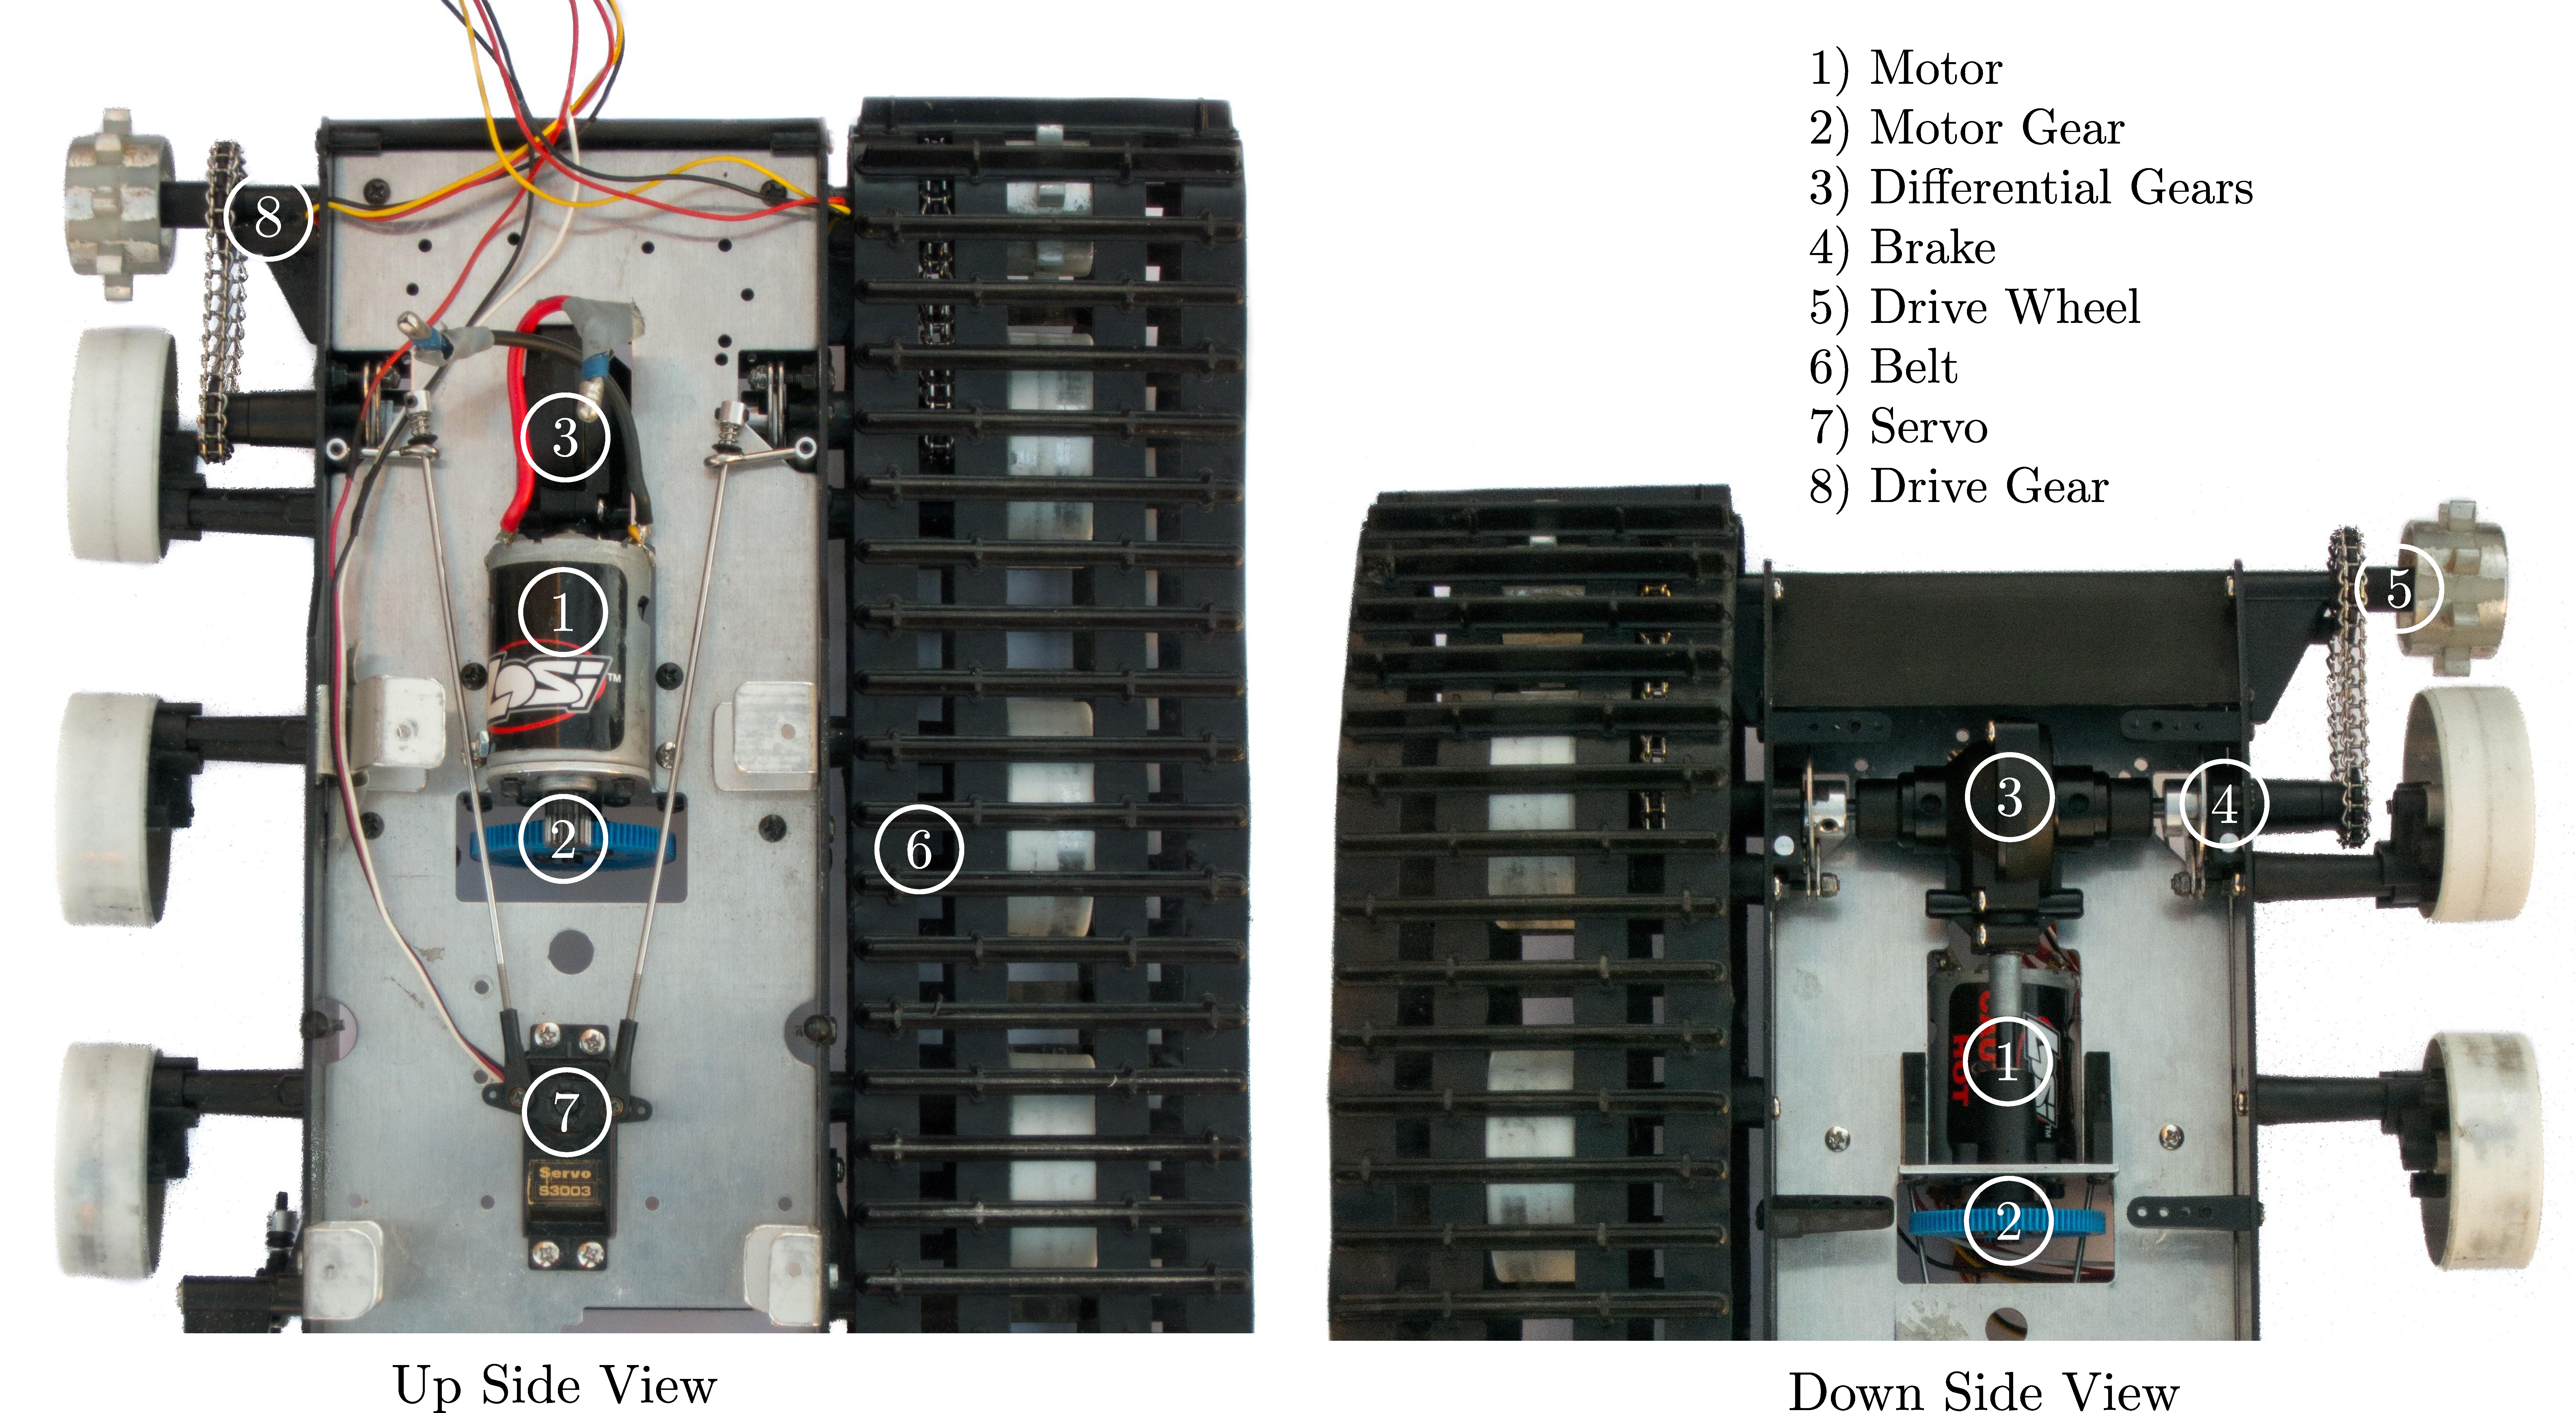
\includegraphics[scale=.09]{figures/FullVehicle.pdf}
	\caption{Picure presenting some of the elements on the vehicle.}
	\label{FullVehicle}
\end{figure}
%\noindent 1) Motor\\2)Motor Gear\\3)Differential Gears\\4) Brakes\\5) Drive Wheel\\6) Belts\\7) Servo

To be able to model this drivetrain, a simplified drawing of the vehicle is made. The drivetrain contains the gear connected to the DC motor, the differential gear box and the gears connected to the belts. The drivetrain is illustrated in \figref{vehicleDescriptionDriveTrain}.

\begin{figure}[H]
	\centering
	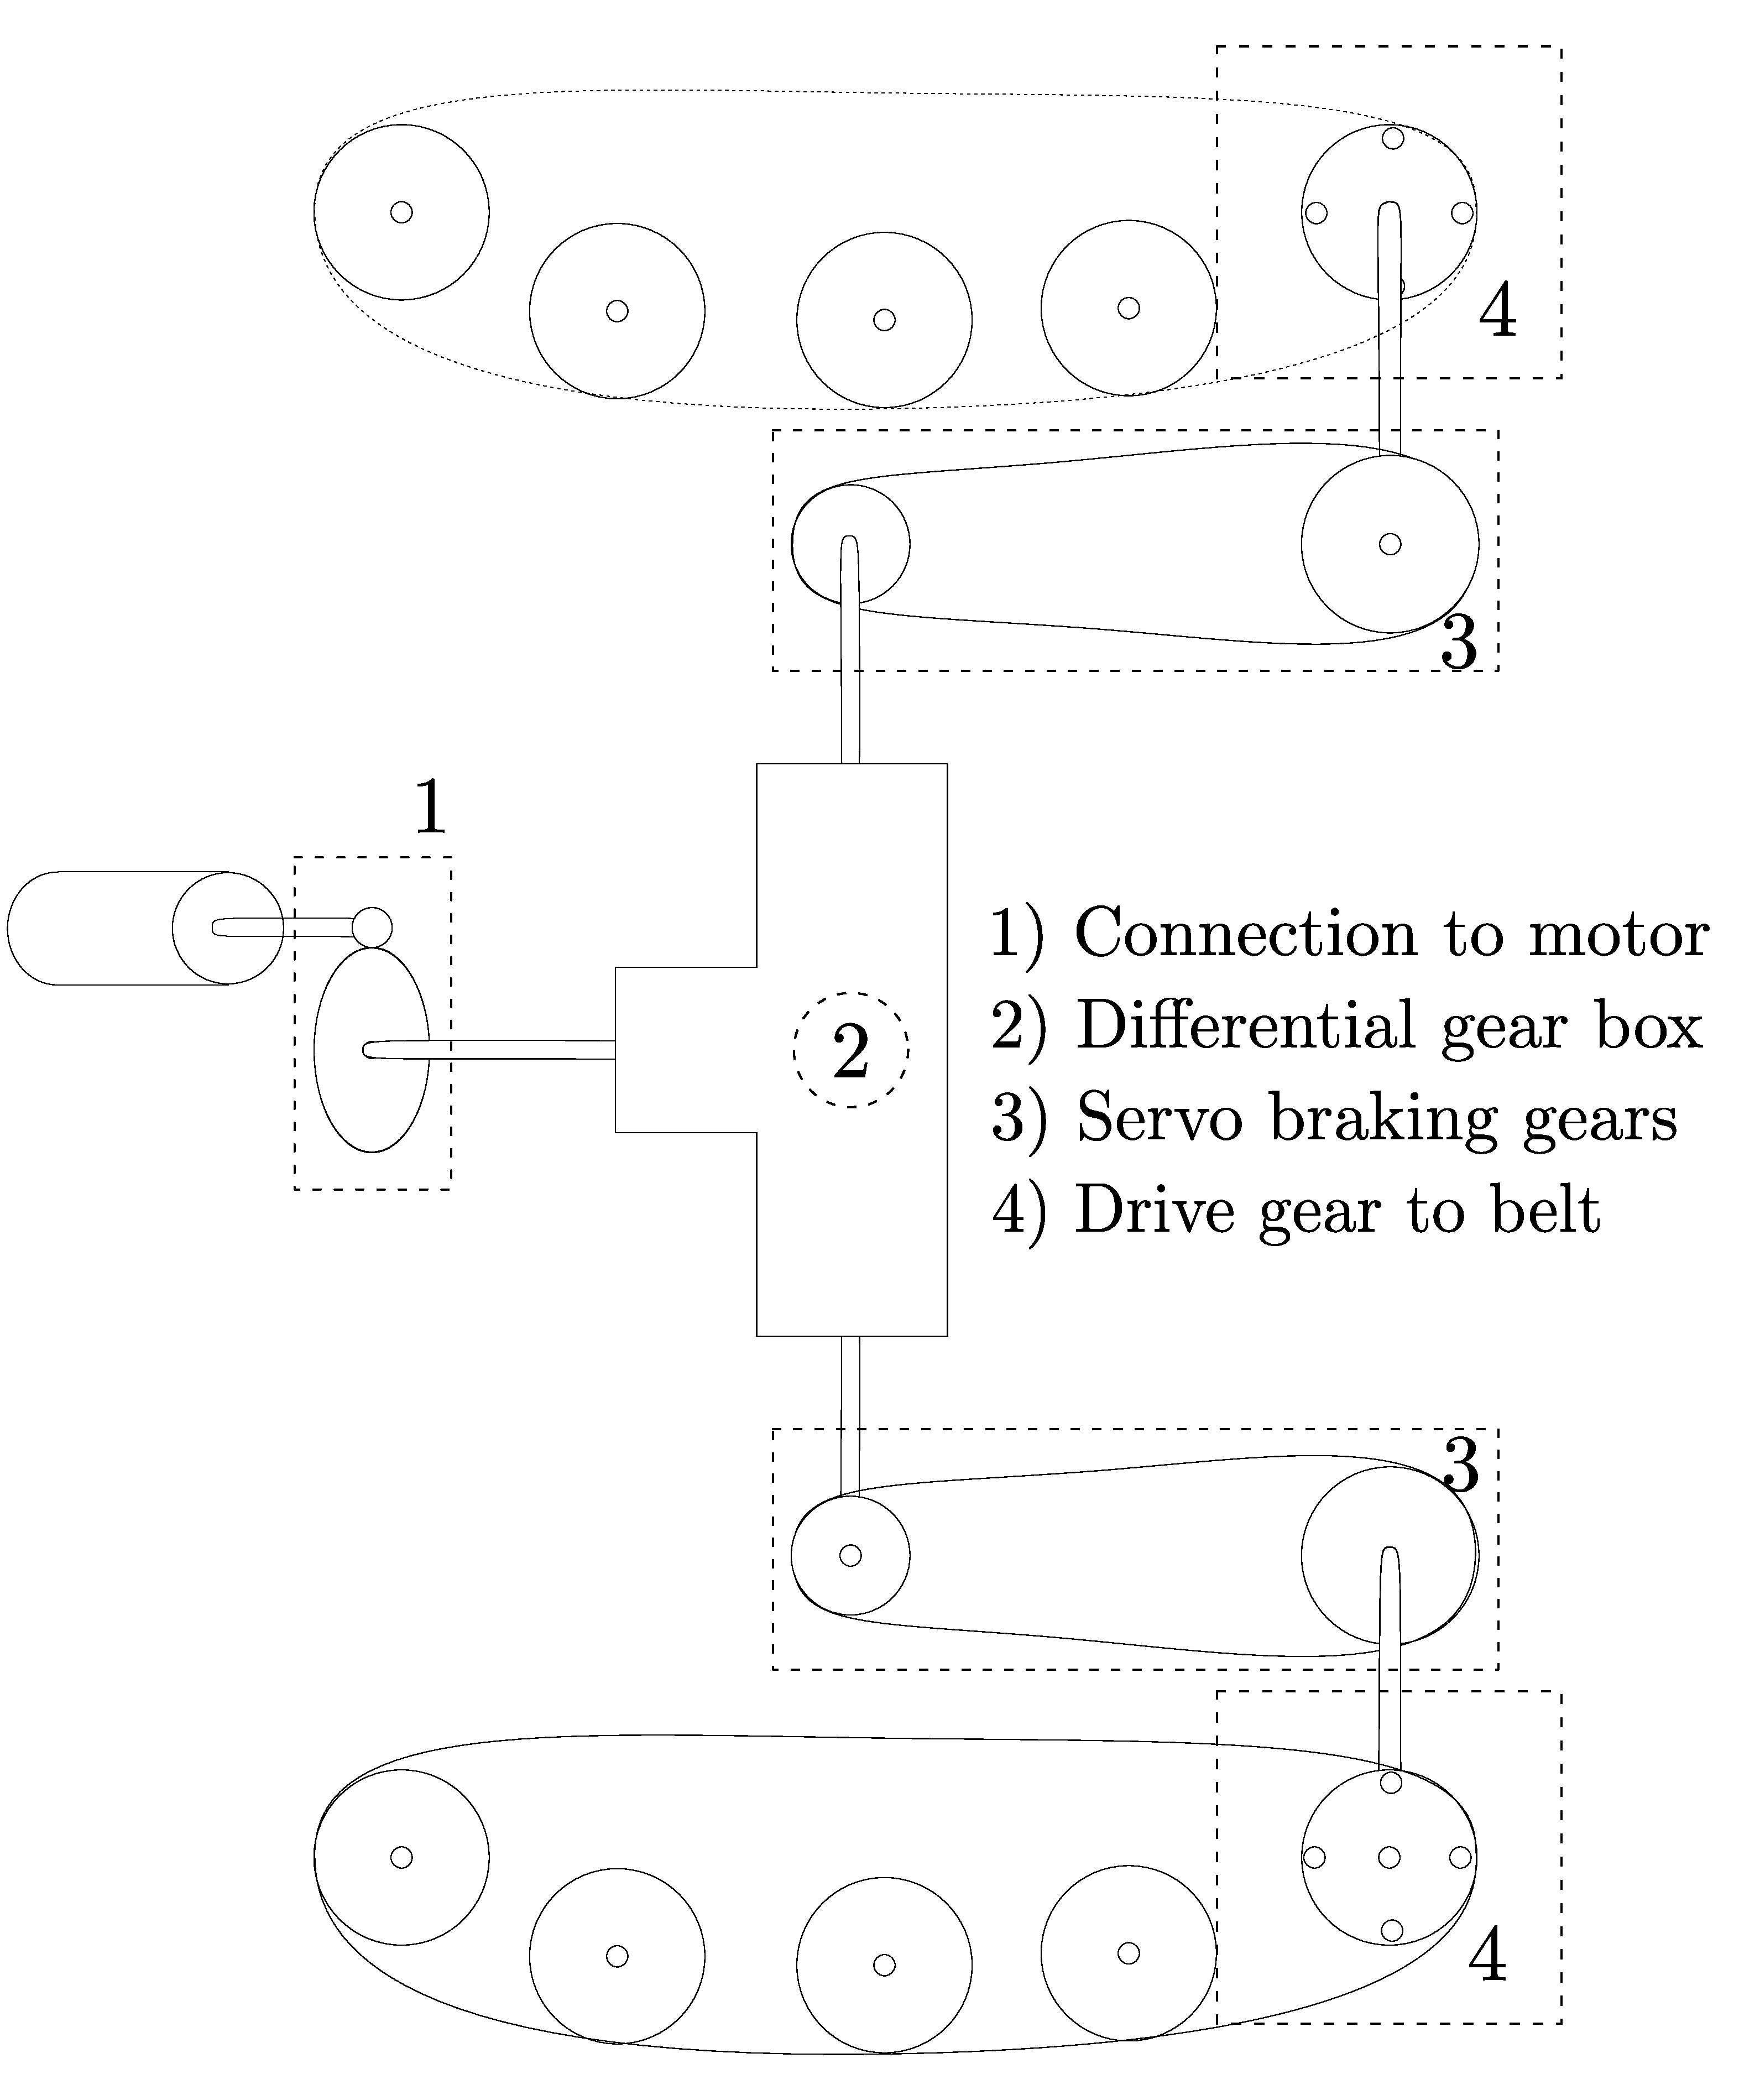
\includegraphics[scale=.25]{figures/vehicleDescriptionDriveTrain.pdf}
	\caption{Illustration of components included in the drivetrain.}
	\label{vehicleDescriptionDriveTrain}
\end{figure}

It is known that the motor(1) delivers a force. This force is delivered to the system through a motor-shaft with a connecting gear(2). This gear is connected to the start of the drivetrain. The gear at the start of the drivetrain is connected, through a shaft, to a differential gear box(3). From the differential gears two shafts are connected to a gear, which transfers a rotational velocity to the drive gears(4).
From there the rotational velocity makes the drive-wheel(5) turn, thus rotating the belts, which are supported by four free wheels on each side. 

In the following segment the differential gears are explained.